%W rozdziale "wydajność" Autor przedstawi stosowane rozwiązania zwiększające wydajność sprzętową systemu, takie jak zestaw rozkazów MMX, AVX oraz możliwości kart graficznych GPU. 
%%
%Ponadto opisana będzie konieczność realizacji kluczowych operacji takich jak: równoległe mnożenie oraz wieloskładnikowe dodawania niezbędne do efektywnego budowania sieci MLP oraz CNN. 
%%
% ********************
\section{ Maszyna Turinga }
Zasada działania maszyny Turinga sprowadza się do cyklicznego wykonywania sekwencji operacji: odczytu wartości z pamięci, wykonaniu działania, zapisaniu wyniku w pamięci. Modelowanie tworu przetwarzającego informacje całą objętością przy użyciu maszyny sekwencyjnej w miarę powiększania modelu spowoduje lawinowy wzrost czasu przetwarzania.
%%
\section{ Szybsze obliczenia grafiki 3D }
W zastosowaniach inżynierskich (oraz rozrywkowych) maszyn liczących bardzo szybko pojawiała się potrzeba realizacji szybkich obliczeń translacji punktów w przestrzeni 3D.
Operacje te sprowadzają się do mnożenia wektora współrzędnych znormalizowanych punktu przez macierz translacji:
\begin{equation*} P =  \begin{bmatrix}
 x\\
 y\\
 z\\
 1
        \end{bmatrix} ,
  T =  \begin{bmatrix}
 1 & 0 & 0 & x\\
 0 & 1 & 0 & y\\
 0 & 0 & 1 & z\\
 0 & 0 & 0 & 1
        \end{bmatrix} ,
  O_x =  \begin{bmatrix}
 1 & 0 & 0 & 0\\
 0 & c & -s & 0\\
 0 & s & c & 0\\
 0 & 0 & 0 & 1
        \end{bmatrix} ,
R =  \begin{bmatrix}
 1 & 0 & 0 & 0\\
 0 & 1 & 0 & 0\\
 0 & 0 & 1 & 0\\
 0 & 0 & 1/d & 0
        \end{bmatrix} 
\end{equation*}

a po rozpisaniu mamy:
\begin{equation*}
\begin{matrix}
  X = x*m[0][0] + y*m[1][0]+z*m[2][0] + w*m[3][0] \\

  Y = x*m[0][1] + y*m[1][1]+z*m[2][1] + w*m[3][1] \\

  Z = x*m[0][2] + y*m[1][2]+z*m[2][2] + w*m[3][2] \\

  W = x*m[0][3] + y*m[1][3]+z*m[2][3] + w*m[3][3]  \\
  \end{matrix}
\end{equation*}
Pierwszą odpowiedzią na to zapotrzebowanie był wprowadzony na rynek w 1980 roku koprocesor arytmetyczny Intel 8087, jego zadaniem było przyspieszenie operacji arytmetycznych zwłaszcza na liczbach zmiennoprzecinkowych w systemach opartych o procesor Intel 8088 i Intel 8086.\newpage
\subsection{ Funkcje procesora MMX, SIMD, SSE, AVX }
SIMD (Single Instruction, Multiple Data) to funkcja procesora, która pozwala wykonywać jedną instrukcję na wielu 'strumieniach'  danych. Może ona ewentualnie zwiększyć wydajność Twoich programów. SIMD to postać przetwarzania równoległego; jednak w niektórych przypadkach przetwarzanie różnych strumieni może odbywać się sekwencyjnie. Pierwszą implementacją był zbiór instrukcji MMX, zastąpiony przez strumieniowe rozszerzenia SIMD (ang. Streaming SIMD Extension, SSE). Później do SSE dodano zaawansowane rozszerzenia wektorowe (ang. Advanced Vector Extension, AVX).\cite{asmx64} 
Procesor obsługujący SSE ma 16 dodatkowych rejestrów 128-bitowych (xmm0-xmm15). Procesor obsługujący AVX2 ma 256-bitowe rejestry ymm, AVX-256 i AVX-10 512-bitowe rejestry zmm.\cite{asmx64} 
\begin{figure}[ht]
	\centering 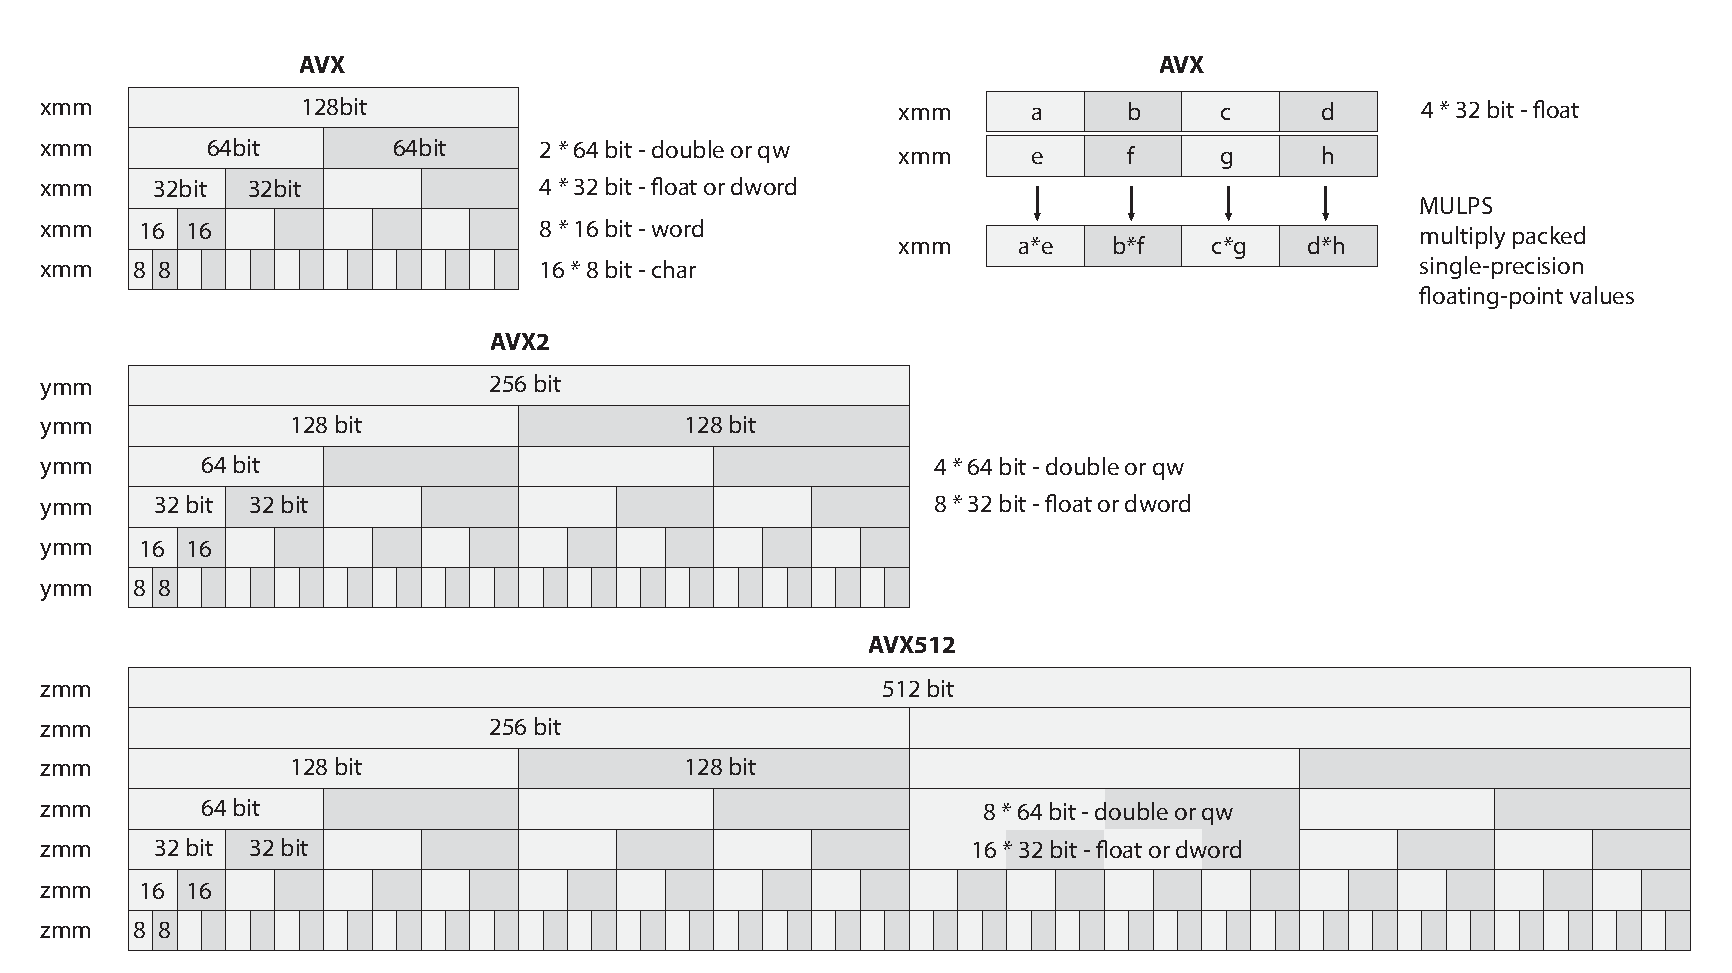
\includegraphics[width=0.99\textwidth]{rysunki/avx.jpg} 
	\caption{ Rejestry AVX, AVX2 i AVX512,operacja równoległego mnożenia AVX}
	\label{rys:modelsztucznegoneuronu}
\end{figure}
Rozkaz MULPS wykonuje jednocześnie jednocześnie 4 mnożenia zestawu 8 liczb 32 bitowych.\newline
Instrukcje w AVX512 VMPADDWD, VMPADDUBSW - wykonują mnożenie wektorowe, następnie dodawanie sąsiednich elementów. \((a_{i}\cdot b_{i}+a_{i+1}\cdot b_{i+1})\)

Funkcje te przyspieszają operacje iloczynu Hadamarda (.*)\cite{WKasprzak} czyli wielokanałowego mnożenia. W zależności od wersji dla zmiennych typu float uzyskano od 4 do 16 kanałów, czyli 16 operacji mnożenia w czasie jednego rozkazu.
\cite{yt_MMX}
\newpage
\section{ Obliczenia na GPU }
\subsection{Równoległe mnożenie}
Wydajne obliczanie iloczynu Hadamarda (.*) wektorów o dużych rozmiarach mogą zapewnić procesory graficzne, w których znajdują się tysiące jednostek obliczeniowych. Czas wykonania kilku tysięcy mnożeń zajmuje tyle samo czasu co wykonanie jednego mnożenia. Użycie kart graficznych przy modelowaniu głębokich sieci jest koniecznością, ponieważ skraca czas trenowania sieci o rzędy wielkości w stosunku do obliczeń na CPU. W niniejszej pracy wykorzystano kartę NVIDIA GeForce RTX 4070 wyposażonej w 5888 rdzeni CUDA oraz 12282 MB pamięci na karcie graficznej. \cite{cuda_} \cite{wroc}\newline
\begin{figure}[ht]
	\centering 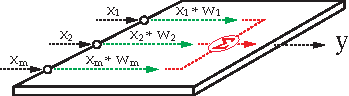
\includegraphics{rysunki/sum_2.jpg} 
	\caption{ Mnożenie równoległe i wielokanałowe dodawanie }
	\label{rys:operacje niezalezne i zalezne}
\end{figure}
\subsection{Wielokanałowe dodawanie}
Sumowanie a+b+c+d realizowane jest analogiczne do zdegenerowanego drzewa binarnego czyli 
(((a+b)+c)+d). Przy dużej ilości składników możemy spróbować zastosować zwykłe drzewo binarne niezdegenerowane, a operacja dodawania może stanie się częściowo równoległa ((a+b) + (c+d).
Maszyny cyfrowe obecnie nie są wyposażone w sumatory wielokanałowe pozwalające dodawać więcej niż 2 liczby jednocześnie. Można zasymulować quasi-równoległe dodawanie stosując nawiasy.
\begin{figure}[h]
	\centering 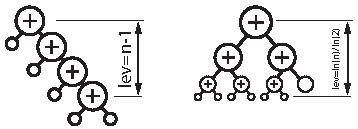
\includegraphics[width=0.6\textwidth]{rysunki/sum.jpg} 
	\caption{ drzewo zdegenerowane i niezdegenerowane}
	\label{rys:operacjesynch}
\end{figure}

\begin{itemize}
    \item \(b=((..((a1+a2)+(a3+a4))+((a5+a6) ...\) 
          czas wykonania: \textbf{0.09568 [sek.]}
    \item \( b=a1+a2+a3+a4+...+a1024\) 
          czas wykonania: \textbf{0.247875 [sek.]}    
\end{itemize}
~\newline
Uzyskamy dwukrotne zwiększenie szybkości przez dodanie nawiasów. Przy 32 składnikach mamy 16 + 8 + 4 + 2 + 1 dodawań, jednak pierwsze 16 może być wykonane równolegle, kolejna 8 także jest od siebie niezależna, podobnie 4 i 2. Czyli dla 32 elementów  mamy 31 dodawań w 5 poziomach. Dla 1024 składników mamy 1023 dodawania, 512+256+128...+1 w 10 poziomach. \cite{cuda_}
\section{Matlab}
Dodatek Parallel computing w Matlab umożliwia wykonywanie obliczeń równolegle, w osobnych wątkach, procesach, a także z wykorzystaniem kart graficznych (obecnie tylko NVidia). Dodatki Optimalization Toolbox i Optimalization Computing Toolbox optymalizują tworzony kod, zwiększając jego wydajność. Dodatek Deep Learning Toolbox dostarcza gotowych metod do obliczeń sieci neuronowych.
\newline
w Matlab karty graficzne (NVidia) są widoczne nawet bez instalowania w systemie dedykowanych sterowników. Karty AMD nie są widoczne.
 